\documentclass[11pt,a4paper,uplatex,dvipdfmx]{ujarticle} 		% for uplatex
%\documentclass[11pt,a4j,dvipdfmx]{jarticle} 					% for platex
%=======================================
% form00_header.tex
%	General header for kakenhiLaTeX,  Moved over from form00_2010_header.tex.
%	2009-09-06 Taku Yamanaka (Osaka Univ.)
%==== General Version History ======================================
% 2006-05-30 Taku Yamanaka (Physics Dept., Osaka Univ.)
% 2006-06-02 V1.0
% 2006-06-14 V1.1 Use automatic calculation for cost tables.
% 2006-06-18 V1.2 Split user's contents and the format.
% 2006-06-20 V1.3 Reorganized user and format files
% 2006-06-25 V1.4 Readjusted all the table column widths with p{...}.
%				With \KLTabR and \KLTabRNum, now the items can be right-justified
%				in the cell defined by p{...}.
% 2006-06-26 V1.5 Use \newlength and \setlength, instead of \newcommand, to define positions.
% 2006-08-19 V1.6 Remade it for 2007 JFY version.
% 2006-09-05 V1.7 Added font declarations suggested by Hoshino@Meisei Univ.
% 2006-09-06 V1.8 Introduced usePDFform flag to switch the form file format.
% 2006-09-09 V1.9 Changed p.7, to allow different heights between years. (Thanks to Ytow.)
% 2006-09-11 V2.0 Added an option to show budget summary.
% 2006-09-13 V2.1 Added an option to show the group.
% 2006-09-14 V2.1.1 Cleaned up Kenkyush Chosho.
% 2006-09-21 V2.2 Generated under a new automatic development system.

% 2007-03-24 V3.0 Switched to a method using "picture" environment.

% 2007-08-14 V3.1 Switched to kakenhi3.sty.
% 2007-09-17 V3.2 Added \KLMaxYearCount
% 2008-03-08 V3.3 Remade it for 2009 JFY version\
% 2008-09-08 V3.4 Added \KLXf ... \KLXh.
% 2011-10-20 V5.0 Use kakenhi5.sty, to utilize array package in tabular environment.
% 2012-08-14 v5.1 Moved preamble and kakenhi5 into the current directory, instead of the parent directory.
% 2012-11-10 v6.0 Switched to kakenhi6.sty.
% 2015-08-26 v6.1 Added KLFirstPageIsLongPage flag.
% 2017-05-27 v7.0 Simplified for the new format.
%=======================================
% Dummy section and subsection commands.
% With these, some editors (such as TeXShop, etc.) can jump to the (sub)sections.
\newcommand{\dummy}{dummy}% 
\renewcommand{\section}[1]{\renewcommand{\dummy}{#1}}

\usepackage{calc}
\usepackage{geometry}                % See geometry.pdf to learn the layout options. There are lots.
\usepackage[dvipdfmx]{graphicx}
\usepackage{color}
\usepackage{ifthen}
\usepackage{udline}
\usepackage{array}
\usepackage{longtable}
\usepackage{fancyhdr}
 % pieces
%==================================================
% kakenhi7.sty
%==================================================
% v1
% Minimum amount of macros for writing Kakenhi forms.
%
% 2005-10-24 Taku Yamanaka, Physics Dept. Osaka Univ.
%		taku@hep.sci.osaka-u.ac.jp
% 		Macros such as XYBC, etc. were imported from Kakenhi Macro at
% 		http://www.yukawa.kyoto-u.ac.jp/contents/researcher/kakenhi.html .
% 2006-06-04 Taku
%		Added macros to draw boxes if \DrawBox is in the source.
%		This is useful when designing the LaTeX forms.
% 2006-06-14 Taku
%		Added LaTeX macros to add costs 
%		(\KLResetGrandSum, \KLCostItem, \KLSum, \KLGrandSum).
%		Added a macro \Number to supply commas every 3 digits (imported from kkh.mac).
% 2006-06-25 Taku
%		Added \KLTabC, \KLTabR, \KLTabRNum to specify alignments in tables.
%		Please note that \phantom{...} is required for the column, 
%		or otherwise somehow p{...mm} is ignored.
% 2006-08-13 Taku
%		Added \KLItemNumUnitCost . This requires calc.sty.
% 2006-09-06 Taku
%		Added KLGrandTotalValue to add ALL the costs.
%		Also added \KLPrintGrandTotal to print the total on the console.
% 2006-09-09 Taku
%		Added macros to handle "efforts".
% 2006-09-10 Taku
%		Added \KLnewcounter to make series of counters.
%		Modified \KLResetGrandSum and \KLSum to add the sum for 
%		each category and year.
% 2006-09-11 Taku
%		Added \NumC to display LaTeX counter with commas.
% 2006-09-12 Taku
%		Added simple macros to make group table.
% 2006-09-23 Taku
%		Added the 'Fair License' notification.
% 2006-10-22 Taku
%		Initialize KLNumPeople to -1, so that the first header row will not be included in the count.
%====================================================
% v2
% 2007-03-24 Taku
%		Instead of using Kakenhi Macros to position items, 
%		switched to a new method using
%		"picture" environment.  The origin of the coordinate is set to 
%		the lower left corner of the paper.  The positions are given in "points", 
%		as can be read by gv. These methods were suggested by 
%		Tsutomu Sakurai at Saitama Univ..
% 2007-03-30 Taku
%		The sum of each category and year is made using 
%		macros \KLItemCost, etc., instead of \KLSum.  This is a step toward
%		automatically aligning category sums in the same year, in some forms.
% 2007-04-02 Taku
%		Added \KLBudgetMiniTabular, \KLMiniSum, etc. to handle
%		budget tables with multiple category columns.
% 2007-05-04 Taku
%		Added \multicolumnDottedLine .
%==================================================
% v3 
% 2007-08-14 Taku
%		Simplified page handling, by introducing \KLBeginSinglePage,
%		\KLPageRange, etc..
% 2007-09-01 Taku
%		Added a new command, \KLItemNumUnitCostLocation , 
%		and \KLAddCost to clean things up.
% 2007-09-06 Taku
%		Set \KLEven/OddLeft/RightEdge parameters in \KLWaterMark.
%		Without it, if \KLLeftEdge or \KLRightEdge is used inside watermark,
%		it generated a very obscure error message, which was hard to track down.
% 2007-09-09 Taku
%		Removed clearring \thiswatermark in \KLClearWaterMarks.
% 2007-09-12 Taku
%		Added \KLPriorityItemNumUnitCostTwo for Tokusui.
% 2007-09-14 Taku
%		Added \KLItemNumUnitCostTwo for tokutei_koubo.
% 2007-09-17 Taku
%		In \KLAddCost, costs are added only if it is within the defined year range.
% 2008-09-02 Taku
%		  Added \KLMonthPriorityItemNumUnitCostTwo for tokutei_keizoku.
% 2008-09-07 Taku
%		   Use \KLJFY to print year in budget tables.
% 2008-10-21 Taku
%			Added KLItemNumUnitCostInParen for shorei.
% 2009-09-03 Taku
%			Added \dottedLine .
%==================================================
% v4
% 2009-09-06 Taku
%			Added macros for partial typesetting.
% 2009-09-12 Taku
%			Added macros for showing coordinates and edges.
% 2009-09-13 Taku
%			Added macros to show boxes and minipage frames and their corner coordinates.
% 2010-03-04 Taku
%			Moved macros for calculating lengths and positions from form07_header.tex to here.
% 2010-04-11 Taku
%			Added \KLItemCostOne for jisedai, and necessary flags to print budget sums before 
%			the detailed budget table.
%==================================================
% v5
% 2011-10-20 Taku
%			By using array package within tabular environment, the following macros were simplified:
%			\KLTabC, \KLTabR, \KLBudgetMiniTabular, 
%			New Macros:
%			\KLCC, \KLCR
% 2011-10-24 Taku
%			Removed using \KLTabR from most of the budget tables.
% 2011-10-26 Taku
%			Added KLMyBudget.
%			Modified KLYearItemNumUnitCostTwo to just put the JFY if the second item is blank.  (For Kiban S)
% 2012-03-10 Taku
%			Changed the tabcolsep for \KLMyBudget to 0pt.
% 2012-08-14 Taku
%			Moved xxx_forms_pdf and _eps directories to under mother.
% 2012-09-09	Taku
%			Added \KLbibitem(B) and \KLcite(B).
% 2012-09-16	Taku
%			Added \KLOtherApplication, \KLOtherApplicationReasons, and \KLOtherFundReasons
%			for tokusui (and maybe for others in the future).
%==================================================
% v6
% 2012-11-10	Taku
% 			Modified \KLOtherApplicationReasons and \KLOtherFundReasons to make the tables compact.
%			These were in hook3.tex for the 2013 version.
%			Added \KLOtherApplicationDiff for many shumokus.
%			Removed \KLbibitemB and \KLciteB.
%			Changed \KLbibitem to use a dedicated column for numbering.
% 2012-11-11	Taku
%			Added \KLItemSetCostLocationInfo and \KLItemCostInfo.
% 2013-09-19	Taku
%			Added \KLOtherPD and \KLOtherPDShort to enter JSPS PD for other funds.
% 2013-10-02	Taku
%			Changed \KLbibItem, not to use a dedicated column for numbering, 
%			because otherwise the label defined in \label{...} cannot be used in @currentlabel.
% 2014-09-22	Taku
%			Added \KLCL for filling narrow tabular cells in English.  
%			(Suggested by Frank Bennett.)
% 2014-11-08	Taku
%			Added an instruction in \KLCheckPageLimit.
% 2015-08-23	Taku
%			Added NumCk to show numbers divided by 1000 (truncated).
% 2015-08-24	Taku
%			Introduced \KLLongPage and \KLSimpleLongPage to offer floating environment in 
%			single-page-frames.
%=====================================================
% v7
%	Frames are gone!  Simplify kakenhiLaTeX to benefit from 
%	the new style.
% 2017-05-03	Taku
%			Added \KLAnotherFund .
% 2017-05-27	Taku
%			Made \KLBeginSubject and \KLEndSubject to handle new 
%			mother file style.
% 2017-08-17 Taku
%	Added \KLItemCostNoYear and \KLEndBudgetNoYear for kokusai_kyoudou.
% 2017-08-19	Taku
%			Updated \KLBeginSubject and \KLEndSubject to handle 
%			various headers.
% 2017-08-20	Taku
%			\KLBeginSubject calls \KLFirstPageStyle and \KLDefaultPageStyle
%			which should be defined for each shumoku (or JSPS/MEXT).
%			This is to pass the subject name etc. to the header.
% 2017-08-27	Taku
%			Set section number in \KLBeginSubject.
% 2017-08-29	Taku
%			Moved over KLShumokuFirstPageStyle and KLShumokuDefaultPageStyle.
%			Added jsps-abs-p1-header, jps-abs-subject-header, and 
%			jsps-abs-default-header as arguments to \KLShumoku***Header.
% 2017-09-02	Taku
%			Added \KLBeginSubjectWithHeaderCommands for more flexible header style.
% 2017-09-03	Taku
%			Added \vspace*{-4mm} after \includegraphics in \KLBeginSubject*.
% 2017-09-05	Taku
%			Removed now-the-old commands.
% 2020-01-02	Taku
%			Added more numbers to \KLJint for gakuhen_a.
% 2020-01-15	Taku
%			Changed the horizontal position (none --> -3mm) 
%			and the width of the top boxes for headers (\linewidth --> 1.02\linewidth)
%			to reproduce the original boxes.  
%			This became necessary because the margins were set correctly in form02_header.tex.
%=====================================================

%=====================================================
% Macro to supply commas every 3 digits (up to 9 digits)
%	Imported from kkh.mac for Kakenhi Macro.
%=====================================================
%
\newif\ifNumWithCommas \NumWithCommastrue
\def\NumWithCommas{\NumWithCommastrue}
\def\NumWithoutCommas{\NumWithCommasfalse}
\newcount\Numa
\newcount\Numb
\def\Numempty{}%output blank if "-0" is given
\def\Number#1{\edef\Numpar{#1}\ifx\Numempty\Numpar\else%
\ifNumWithCommas\Numa=#1\relax
\ifnum\Numa>999999\divide\Numa by 1000000
\number\Numa,%
\multiply\Numa by -1000000\advance\Numa by #1\relax
\Numb=\Numa\divide\Numa by 1000
\ifnum\Numa<100 \ifnum\Numa<10 0\fi0\fi\number\Numa,%
\multiply\Numa by -1000\advance\Numa by \Numb
\ifnum\Numa<100 \ifnum\Numa<10 0\fi0\fi\number\Numa%
\else\ifnum\Numa>999\divide\Numa by 1000
\number\Numa,%
\multiply\Numa by -1000\advance\Numa by #1\relax
\ifnum\Numa<100 \ifnum\Numa<10 0\fi0\fi\number\Numa%
\else\number\Numa\fi\fi\else\number#1\fi\fi}

%======================================================
% Macro to display LaTeX counter with commas every 3 digits.
%======================================================
\newcommand{\NumC}[1]{\Number{\value{#1}}}

\newcounter{kyen}
\newcommand{\NumCk}[1]{%
	\setcounter{kyen}{\arabic{#1}/1000}
	\Number{\value{kyen}}
}

%======================================================
% Macros to align (right-justify, center) elements within a tabular cell
% whose width is defined by p{...}.
% 2006-06-25 Taku
% 	These are necessary, because the cell width should be given explicitly
% 	by p{...mm} to match the given table in a tabular environment.  
% 	One could allocate a width with \phantom{...},
% 	but it is a little tricky, since it depends on the font size.
%======================================================

%---------------------------------------------------------------------
% Center text within a tabular cell allocated by p{...}
%\newcommand{\KLTabC}[1]{\multicolumn{1}{c}{#1}}
\newcommand{\KLTabC}[1]{\centering\arraybackslash#1}
% This new method does not require a dummy table row to put them in correct columns.
%
% This should be used in tabular definition, as:
%	\begin{tabular}[t]{>{\KLCC}p{30pt}p{50pt}}
\newcommand{\KLCC}{\centering\arraybackslash}

%---------------------------------------------------------------------
% Right justify text within a tabular cell allocated  by p{...}
%\newcommand{\KLTabR}[1]{\multicolumn{1}{r@{\ }}{#1}}
\newcommand{\KLTabR}[1]{\raggedleft\arraybackslash#1}

% This should be used in tabular definition, as:
%	\begin{tabular}[t]{>{\KLCR}p{30pt}p{50pt}}
\newcommand{\KLCR}{\raggedleft\arraybackslash}%

%---------------------------------------------------------------------
% Right justify number (with comma every 3 digits) 
% within a tabular cell allocated by p{...}
\newcommand{\KLTabRNum}[1]{\KLTabR{\Number{#1}}}

%---------------------------------------------------------------------
% Left justify text within a tabular cell allocated by p{...}
% This should be used in tabular definition, as:
%	\begin{tabular}[t]{>{\KLCL}p{30pt}p{50pt}}
\newcommand{\KLCL}{\raggedright\arraybackslash}%

%=================================================
%  counter tools
%=================================================
\newcounter{KLtmp}

%------------------------------------------------------------------------------
% Makes a set of counters, with prefix #1, followed by 
% suffix ranging from 0 to #2 - 1.
% For example, \KLnewcounter{mine}{3} makes counters
% mine0, mine1, and mine2 .
%-------------------------------------------------------------------------------
\newcommand{\KLnewcounter}[2]{
	\setcounter{KLtmp}{0}
	
	\whiledo{\value{KLtmp} < #2}{
		\newcounter{#1\arabic{KLtmp}}
		\stepcounter{KLtmp}
	}
}

%------------------------------------------------------------------------------
% Dumps the contents of the counters.
%------------------------------------------------------------------------------
\newcommand{\KLdumpcounter}[2]{
	\setcounter{KLtmp}{0}
	
	\whiledo{\value{KLtmp} < #2}{
		#1\arabic{KLtmp} : \arabic{#1\arabic{KLtmp}}\\
		\stepcounter{KLtmp}
	}
}

%=======================================================
% LaTeX macros to add costs.
%	2006-06-14 Taku Yamanaka
%=======================================================
\newcounter{KLCost}				% to calculate cost = #units x unit cost
\newcounter{KLGrandTotalValue}		% for the grand total of all the categories in all years
\setcounter{KLGrandTotalValue}{0}

\newcommand{\KLCostCategory}{KLequipments}
\newcounter{KLYearCount}
\newcounter{KLPrintYear}

% Make counters for annual sums for each category-----------------------
\newcommand{\KLMaxYear}{8}
\KLnewcounter{KLequipments}{\KLMaxYear}
\KLnewcounter{KLexpendables}{\KLMaxYear}
\KLnewcounter{KLdomestic}{\KLMaxYear}
\KLnewcounter{KLforeign}{\KLMaxYear}
\KLnewcounter{KLtravel}{\KLMaxYear}
\KLnewcounter{KLgratitude}{\KLMaxYear}
\KLnewcounter{KLmisc}{\KLMaxYear}
\KLnewcounter{KLAnnualSum}{\KLMaxYear}

%------------------------------------------------
% Add up the given cost to category-year sum, category sum, year-sum, and total.
% 2007-09-01 Taku
% 2007-09-17 Taku: Add costs only if it is within the defined year range.
%------------------------------------------------
\newcommand{\KLAddCost}[1]{%
	\ifthenelse{\value{KLYearCount} > \value{KLMaxYearCount}}{%
		%pass
	}{%
		\addtocounter{\KLCostCategory0}{#1}%
		\addtocounter{\KLCostCategory\arabic{KLYearCount}}{#1}%
		\addtocounter{KLAnnualSum\arabic{KLYearCount}}{#1}%
		\addtocounter{KLAnnualSum0}{#1}%
		\ifthenelse{\equal{\KLCostCategory}{KLdomestic}}{%
			\addtocounter{KLtravel0}{#1}%
			\addtocounter{KLtravel\arabic{KLYearCount}}{#1}%
		}{}%
		\ifthenelse{\equal{\KLCostCategory}{KLforeign}}{%
			\addtocounter{KLtravel0}{#1}%
			\addtocounter{KLtravel\arabic{KLYearCount}}{#1}%
		}{}%
	}%
}


\newcommand{\KLClearWaterMarks}{%
	%--empty watermarks
	\watermark{}
%	\thiswatermark{}
	\rightwatermark{}
	\leftwatermark{}
}

\newcommand{\KLInput}[1]{%	The macros defined inside the file are only valid within the file.
	\begingroup
	\input{#1}
	\endgroup
}

%================================
% For 2017 new style without frames
%================================
\newcommand{\KLShumokuFirstPageStyle}[5]{%
%	Defines the header for the first page.
%	Called from \KLBeginSubject.
%--------------------------------
%	#1: page style name
%	#2: 様式
%	#3: 研究種目名
%	#4: 項目名
%	#5: sectionNo
%--------------------------------
	\ifthenelse{\equal{#1}{jsps-p1-header}}{%
		\JSPSVeryFirstPageStyle{#1}{#2}{#3}{#4}{#5}
	}{%
		\ifthenelse{\equal{#1}{jsps-abs-p1-header}}{%
			\JSPSVeryFirstPageStyle{#1}{#2}{#3 概要}{#4}{#5}
		}{%
            		\ifthenelse{\equal{#1}{jsps-subject-header}}{%
            			\JSPSFirstSubjectPageStyle{#1}{#2}{#3}{#4}{#5}
            		}{%
				\ifthenelse{\equal{#1}{jsps-abs-subject-header}}{%
            				\JSPSFirstSubjectPageStyle{#1}{#2}{#3 概要}{#4}{#5}
				}{%
                    			\thispagestyle{#1}
				}
            		}
		}
	}
}

\newcommand{\KLShumokuDefaultPageStyle}[5]{%
%	Defines the default header.
%	Called from \KLBeginSubject.
%--------------------------------
%	#1: page style name
%	#2: 様式
%	#3: 研究種目名
%	#4: 項目名
%	#5: sectionNo
%--------------------------------
	\ifthenelse{\equal{#1}{jsps-default-header}}{%
		\JSPSDefaultPageStyle{#1}{#2}{#3}{#4}{#5}
	}{%
		\ifthenelse{\equal{#1}{jsps-abs-default-header}}{%
			\JSPSDefaultPageStyle{#1}{#2}{#3 概要}{#4}{#5}
		}{%
            		\pagestyle{#1}
		}
	}
}

\newcommand{\KLSubjectName}{}
\newcommand{\KLSubjectMaxPages}{}
\newcommand{\KLSubjectEndPage}{}
\newcounter{KLSubjectEndPage}
\setcounter{KLSubjectEndPage}{0}

\newcommand{\KLSubjectCheckNPages}{%
%	\arabic{page}, \arabic{KLSubjectEndPage}\\
	\ifthenelse{\value{page}>\value{KLSubjectEndPage}}{
		{\LARGE「\KLSubjectName」は \KLSubjectMaxPages\ ページ以内で書いてください。}
		\clearpage
	}{%
	}
}

\newcommand{\KLSubjectAdvancePages}{%
	\renewcommand{\KLSubjectEndPage}{\value{KLSubjectEndPage}}
	\ifthenelse{\value{page}<\KLSubjectEndPage}{%
		\phantom{x}\clearpage
	}{}
	% Advance page if necessary
	\ifthenelse{\value{page}<\KLSubjectEndPage}{%
		\phantom{x}\clearpage
	}{}
	% Advance page if necessary
	\ifthenelse{\value{page}<\KLSubjectEndPage}{%
		\phantom{x}\clearpage
	}{}
	% Advance page if necessary
	\ifthenelse{\value{page}<\KLSubjectEndPage}{%
		\phantom{x}\clearpage
	}{}
	% Advance page if necessary
	\ifthenelse{\value{page}<\KLSubjectEndPage}{%
		\phantom{x}\clearpage
	}{}
}	

\newcommand{\KLJInt}[1]{%
% Returns full-width numerical character.
	\ifthenelse{\equal{#1}{1}}{1}{%
	\ifthenelse{\equal{#1}{2}}{2}{%
	\ifthenelse{\equal{#1}{3}}{3}{%
	\ifthenelse{\equal{#1}{4}}{4}{%
	\ifthenelse{\equal{#1}{5}}{5}{%
	\ifthenelse{\equal{#1}{6}}{6}{%
	\ifthenelse{\equal{#1}{7}}{7}{%
	\ifthenelse{\equal{#1}{8}}{8}{%
	\ifthenelse{\equal{#1}{9}}{9}{%
	\ifthenelse{\equal{#1}{10}}{10}{%
	\ifthenelse{\equal{#1}{11}}{11}{%
	\ifthenelse{\equal{#1}{12}}{12}{%
	\ifthenelse{\equal{#1}{13}}{13}{%
	\ifthenelse{\equal{#1}{14}}{14}{%
	\ifthenelse{\equal{#1}{15}}{15}{%
	\ifthenelse{\equal{#1}{16}}{16}{%
	\ifthenelse{\equal{#1}{17}}{17}{%
	#1}}}}}}}}}}}}}}}}}%
}


\newcommand{\KLBeginSubject}[8]{%
%----------------------------------------------------
%	#1: subjectNo
%	#2: sectionNo
%	#3: sectionJ
%	#4: maxPages
%	#5: pageLengthStyle ('V' for variable, 'F' for fixed)
%	#6: pageCounter (set page counter to this value if the argument exists.
%	#7: subjectFirstPageHeader (header for the first page)
%	#8: defaultPageHeader
%----------------------------------------------------
	\setcounter{section}{#2}
	\setcounter{subsection}{0}
	\setcounter{subsubsection}{0}
	\renewcommand{\KLSubjectName}{#3}
	\renewcommand{\KLSubjectMaxPages}{#4}
	
	\ifthenelse{\equal{#6}{}}{%
	}{%
		\setcounter{page}{#6}
	}
	
	\setcounter{KLSubjectEndPage}{\value{page}}
	\addtocounter{KLSubjectEndPage}{#4}
	
	\ifthenelse{\equal{#7}{}}{%
		% pass
	}{%
		\KLShumokuFirstPageStyle{#7}{\様式}{\研究種目header}{#3}{#2}
	}
	
	\ifthenelse{\equal{#8}{}}{%
		% pass
	}{%
		\KLShumokuDefaultPageStyle{#8}{\様式}{\研究種目header}{#3}{#2}
	}
	
	\noindent
	\hspace{-3mm}
	\includegraphics[width=1.03\linewidth]{subject_headers/\KLYoshiki_#1.pdf}\\
	\vspace*{-4mm}
}

\newcommand{\KLNullHeader}[5]{}
% Dummy command for No header.
% This was introduced to avoid error caused in statement \ifthenelse{\equal{#8}{}} .

\newcommand{\KLBeginSubjectWithHeaderCommands}[8]{%
%----------------------------------------------------
%	#1: subjectNo
%	#2: sectionNo
%	#3: sectionJ
%	#4: maxPages
%	#5: pageLengthStyle ('V' for variable, 'F' for fixed)
%	#6: pageCounter (set page counter to this value if the argument exists.
%	#7: LaTeX command for subjectFirstPageHeader (header for the first page)
%	#8: LaTeX command for defaultPageHeader
%----------------------------------------------------
	\setcounter{section}{#2}
	\setcounter{subsection}{0}
	\setcounter{subsubsection}{0}
	\renewcommand{\KLSubjectName}{#3}
	\renewcommand{\KLSubjectMaxPages}{#4}
	
	\ifthenelse{\equal{#6}{}}{%
	}{%
		\setcounter{page}{#6}
	}
	
	\setcounter{KLSubjectEndPage}{\value{page}}
	\addtocounter{KLSubjectEndPage}{#4}
	
	#7{#7}{\様式}{\研究種目header}{#3}{#2}
	#8{#8}{\様式}{\研究種目header}{#3}{#2}
	
	\noindent
	\hspace{-3mm}
	\includegraphics[width=1.03\linewidth]{subject_headers/\KLYoshiki_#1.pdf}\\
	\vspace*{-4mm}
}

\newcommand{\KLEndSubject}[1]{%
%	#1: pageLengthStyle ('V' for variable, 'F' for fixed)
		\clearpage % This should be done to update page counter for checking.
		\KLSubjectCheckNPages
		\ifthenelse{\equal{#1}{F}}{%
			\KLSubjectAdvancePages
		}{%
		}
}

%==================================================
% Miscellaneous macros
%==================================================

%----------------------------------------------------------------------
% Draw dotted lines across a multiple column table
%----------------------------------------------------------------------
\newcommand{\multicolumnDottedLine}[1]{%
%	\multicolumn{#1}{@{\hspace{-2mm}}c}{\dotfill}\\%
	\multicolumn{#1}{@{}c}{\dotfill}\\%
}

\newcommand{\dottedLine}{%
	\\\noindent
	\dotfill\\
}

%----------------------------------------------------------------------
% Solid line
%----------------------------------------------------------------------
\newlength{\KLLineLength}
\newcommand{\solidLine}[1]{
%----------- keep an empty line between here and \noindent so that it works after normal text and list.

	\noindent
	\hspace*{-10pt}
	\rule[10pt]{\textwidth}{#1}% #1 = 0.5pt, ....
	\vspace*{-10pt}
}

\newcommand{\KLLine}{%
	\solidLine{1pt}
}

%----------------------------------------------------------------------
% publication list (Thanks to Tetsuo Iwakuma [bulletin board #876])
%----------------------------------------------------------------------
\newcounter{KLBibCounter}

\makeatletter	
	\newcommand{\KLbibitem}{%
		\stepcounter{KLBibCounter}%
		\let \@currentlabel \theKLBibCounter
		\arabic{KLBibCounter}. %
	}
\makeatother

\newcommand{\KLcite}[1]{[\ref{#1}]}

%==================================================
%Fair License

%<Copyright Information>

%Usage of the works is permitted provided that this
%instrument is retained with the works, so that any entity
%that uses the works is notified of this instrument.

%DISCLAIMER: THE WORKS ARE WITHOUT WARRANTY.

%[2004, Fair License: rhid.com/fair]
%==================================================
% You may edit/modify this package at your own risk.
% If there are important fixes or changes that you think should be 
% reflected in the standard distribution, please notify:
%	taku@hep.sci.osaka-u.ac.jp  .
%==================================================
 % pieces
% form01_header.tex
% 2017-05-28 Split from form00_header.tex to move \input{kakenhiLaTeX7.sty} to mother_1.tex.
% 2010-01-15 Adjusted margins.
% ===== Parameters for KL (Kakenhi LaTeX) ========================
%%\geometry{noheadfoot,scale=1}  %scale=1 resets margins to 0
\setlength{\unitlength}{1pt}

\newlength{\KLCella}
\newlength{\KLCellb}
\newlength{\KLCellc}
\newlength{\KLCelld}
\newlength{\KLCelle}
\newlength{\KLCellf}

\newcounter{KLMaxYearCount}	% # of years for the proposal
\newcommand{\KLCLLang}{}	% language-dependent left-justification in tabular

% ===== format and header =========
% 2020-01-15: Reset it to match the margins (25 mm on sides, 20 mm on top and bottom). 
% A4: 294 mm x 210 mm.  
% LaTeX's default margin is 1 inch = 25.4 mm.
\setlength{\oddsidemargin}{-1pt}	% (25.0 - 25.4) / 25.4 * 72 pt/inch = -1 pt
\setlength{\evensidemargin}{-1pt}
\setlength{\textwidth}{453pt}		% (210 - 25*2) / 25.4 * 72 = 453 pt
\setlength{\topmargin}{-61pt}	% This and \headheight determine the actual top margin
\setlength{\textheight}{254mm}		% (294 - 20*2) = 254 mm

\setlength{\headheight}{48pt}
\setlength{\headsep}{3pt}

\cfoot{}
\renewcommand{\headrulewidth}{0pt}

\pagestyle{empty}
% ==== other applications table =========
\newcommand{\KLTableHeaderFont}{\fontsize{8.2}{11}\selectfont}
\newcommand{\KLTableHeaderSmallFont}{\fontsize{7.5}{10}\selectfont}
\newcommand{\KLTableHeaderSmallerFont}{\fontsize{7}{10}\selectfont}

 % pieces
% ===== Global year-dependent definitions for the Kakenhi form ===========
% 基本情報
\newcommand{\研究開始年度}{2021}
\newcommand{\研究開始元号年度}{03}	%令和

\newcommand{\一年目西暦}{2021}
\newcommand{\二年目西暦}{2022}
\newcommand{\三年目西暦}{2023}
\newcommand{\四年目西暦}{2024}
\newcommand{\五年目西暦}{2025}
\newcommand{\六年目西暦}{2026}

\newcommand{\一年目}{3}
\newcommand{\二年目}{4}
\newcommand{\三年目}{5}
\newcommand{\四年目}{6}
\newcommand{\五年目}{7}
\newcommand{\六年目}{8}

\newcommand{\一年目J}{3}
\newcommand{\二年目J}{4}
\newcommand{\三年目J}{5}
\newcommand{\四年目J}{6}
\newcommand{\五年目J}{7}
\newcommand{\六年目J}{8}


 % pieces
% hook3: after including packages ===================
 % pieces
%#Name: gakuhen_a_koubo
% form04_jsps_headers.tex
% 2017-08-20 Taku
% 2017-08-29 Taku
%			Added a check against jsps-abs-p1-header.
% 2017-09-02 Taku
%			Added sectionNo to the commands to make them compatible with 
%			\KLBeginSubjectWithHeaderCommands.
%			Use \KLJInt.
% 2018-09-01 Taku
%			Adjusted the heights of the headers by inserting \vspace{-3pt} and \rule.
%
\newcommand{\headerfont}{\fontsize{11}{11}\selectfont}
% ===== Headers =====================================
\newcommand{\JSPSVeryFirstPageStyle}[5]{%
%	Defines the header for the very first page of the form.
%	Called from \KLShumokuFirstPageStyle in form04_***.
%--------------------------------
%	#1: page style name
%	#2: 様式
%	#3: 研究種目名
%	#4: 項目名
%	#5: sectionNo
%--------------------------------
	\fancypagestyle{JSPSVeryFirstPageStyle}{% The name is not taken from #1, because 
		\fancyhf{}
		\fancyhead[L]{\hspace{-37pt}\headerfont#2\ 研究計画調書(添付ファイル項目)\\
				\rule{0pt}{18pt}\\}
%				\rule{0pt}{0pt}\\}
		\fancyhead[R]{\headerfont\textbf{#3\ \KLJInt{\thepage}}\vspace{-5pt}\\
			\rule{0pt}{0pt}\\}
%		\fancyhead[R]{\headerfont\textbf{#3\ \KLJInt{\thepage}\\}}
	}
	\thispagestyle{JSPSVeryFirstPageStyle}
}

\newcommand{\JSPSFirstSubjectPageStyle}[5]{%
%	Defines the header for the first page for the subject.
%	Called from \KLShumokuFirstPageStyle in form04_***.
%--------------------------------
%	#1: page style name
%	#2: 様式
%	#3: 研究種目名
%	#4: 項目名
%	#5: sectionNo
%--------------------------------
	\fancypagestyle{JSPSFirstSubjectPageStyle}{%
		\fancyhf{}
		\fancyhead[R]{\headerfont\textbf{#3\ \KLJInt{\thepage}}\vspace{-5pt}\\
			\rule{0pt}{0pt}\\}
%		\fancyhead[R]{\headerfont\textbf{#3\ \KLJInt{\thepage}\\}}
	}
	\thispagestyle{JSPSFirstSubjectPageStyle}
}

\newcommand{\JSPSDefaultPageStyle}[5]{%
%	Defines the default header for the subject.
%	Called from \KLShumokuDefaultPageStyle in form04_***.
%--------------------------------
%	#1: page style name
%	#2: 様式
%	#3: 研究種目名
%	#4: 項目名
%	#5: sectionNo
%--------------------------------
	\fancypagestyle{JSPSDefaultPageStyle}{%
		\fancyhf{}
		\fancyhead[L]{\headerfont\textbf{【#4(つづき)\ 】}\vspace{-7pt}\\}
		\fancyhead[R]{\headerfont\textbf{#3\ \KLJInt{\thepage}}\vspace{-5pt}\\
			\rule{0pt}{0pt}\\}
%		\fancyhead[R]{\headerfont\textbf{#3\ \KLJInt{\thepage}\\}}	
        }
        \pagestyle{JSPSDefaultPageStyle}
}

 % pieces
%form04_mext_headers_2020
%%\setlength{\oddsidemargin}{-18pt}
%%\setlength{\evensidemargin}{-18pt}
%%\setlength{\textwidth}{486pt}
%%
\newcommand{\mextPageUnderline}{\underline}	
% shingaku_field has no underline under the page #, but others do.  Sigh...
% This will be redefined in form04_shingaku_field_header.tex.	2017-09-03 Taku

\newcommand{\mextPageLF}{}
% page # for shingaku_keikaku is at the bottom of the header.
% page # for shingaku_koubo is one line above the header bottom.

% How come MEXT forms have no unified format??  It is a matter of sense of beauty...
\fancypagestyle{mext-p1-sameline-header}{%
	\fancyhf{}
	\fancyhead[L]{\headerfont\textbf{\様式 (応募内容ファイル (添付ファイル項目))}}
	\fancyhead[R]{\headerfont\textbf{\mextPageUnderline{\研究種目header−\KLJInt{\thepage}}}}
}

\fancypagestyle{mext-p1-offset-header}{%
	\fancyhf{}
	\fancyhead[L]{\headerfont\textbf{\様式 (応募内容ファイル (添付ファイル項目))}\\
			\rule{0pt}{0pt}\mextPageLF}
	\fancyhead[R]{\headerfont\textbf{\mextPageUnderline{\研究種目header−\KLJInt{\thepage}}}\mextPageLF}
}

\fancypagestyle{mext-p1-offset2-header}{%
	\fancyhf{}
	\fancyhead[L]{\headerfont\textbf{\様式 (応募内容ファイル (添付ファイル項目))}\\
			\rule{0pt}{15pt}\\\mextPageLF}
	\fancyhead[R]{\headerfont\textbf{\mextPageUnderline{\研究種目header−\KLJInt{\thepage}}}\mextPageLF}
}

\newcommand{\MEXTVeryFirstPageStyle}[5]{%
%	Defines the header for the very first page of the form.
%	Called from \KLShumokuFirstPageStyle in form04_***.
%--------------------------------
%	#1: page style name
%	#2: 様式 研究計画調書 (**)
%	#3: 研究種目名
%	#4: 項目名
%	#5: sectionNo
%--------------------------------
	\fancypagestyle{JSPSVeryFirstPageStyle}{% The name is not taken from #1, because 
		\fancyhf{}
		\fancyhead[L]{\hspace{-37pt}\headerfont#2\ (添付ファイル項目)\\
				\rule{0pt}{18pt}\\}
%				\rule{0pt}{0pt}\\}
		\fancyhead[R]{\headerfont\textbf{#3\ \KLJInt{\thepage}}\vspace{-5pt}\\
			\rule{0pt}{0pt}\\}
%		\fancyhead[R]{\headerfont\textbf{#3\ \KLJInt{\thepage}\\}}
	}
	\thispagestyle{JSPSVeryFirstPageStyle}
}



\newcommand{\MEXTFieldVeryFirstHeaderWithSectionNo}[5]{%
%	Defines the the very first header for MEXT shingaku_field form in form XXXX-N-n.
%--------------------------------
%	#1: page style name
%	#2: 様式
%	#3: 研究種目名
%	#4: 項目名
%	#5: sectionNo
%--------------------------------
	\fancypagestyle{MEXTFieldVeryFirstHeaderWithSectionNo}{%
		\fancyhf{}
		\fancyhead[L]{\headerfont\textbf{#2(「領域計画書」応募内容ファイル(添付ファイル項目))}\\
				\rule{0pt}{18pt}\\}
		\fancyhead[R]{\headerfont\textbf{\mextPageUnderline{#3−\KLJInt{#5}−\KLJInt{\thepage}}}\mextPageLF}
	}
	\thispagestyle{MEXTFieldVeryFirstHeaderWithSectionNo}
}

\newcommand{\MEXTDefaultHeaderWithSectionNo}[5]{%
%	Defines the default header for MEXT forms in form XXXX-N-n.
%--------------------------------
%	#1: page style name
%	#2: 様式
%	#3: 研究種目名
%	#4: 項目名
%	#5: sectionNo
%--------------------------------
	\fancypagestyle{MEXTDefaultHeaderWithSectionNo}{%
		\fancyhf{}
		\fancyhead[R]{\headerfont\textbf{\mextPageUnderline{#3−\KLJInt{#5}−\KLJInt{\thepage}}}\mextPageLF}
	}
	\pagestyle{MEXTDefaultHeaderWithSectionNo}
}

\newcommand{\MEXTDefaultHeaderWithParenthesis}[5]{%
%	Defines the default header for MEXT forms in form XXXX-N-(n).
%--------------------------------
%	#1: page style name
%	#2: 様式
%	#3: 研究種目名
%	#4: 項目名
%	#5: sectionNo
%--------------------------------
	\fancypagestyle{MEXTDefaultHeaderWithParenthesis}{%
		\fancyhf{}
		\fancyhead[R]{\headerfont\textbf{\mextPageUnderline{#3\KLJInt{#5}−(\KLJInt{\thepage})}}\mextPageLF}
	}
	\pagestyle{MEXTDefaultHeaderWithParenthesis}
}

\newcommand{\MEXTDefaultHeader}[5]{%
%	Defines the default header for MEXT forms in form XXXX-n.
%--------------------------------
%	#1: page style name
%	#2: 様式
%	#3: 研究種目名
%	#4: 項目名
%	#5: sectionNo
%--------------------------------
	\fancypagestyle{MEXTDefaultHeader}{%
		\fancyhf{}
		\fancyhead[R]{\headerfont\textbf{\mextPageUnderline{#3−\KLJInt{\thepage}}}\mextPageLF}
	}
	\pagestyle{MEXTDefaultHeader}
}

%%\newcommand{\MEXTDefaultPageStyle}[5]{%
%%%	Defines the default header for the subject.
%%%	Called from \KLShumokuDefaultPageStyle in form04_***.
%%%--------------------------------
%%%	#1: page style name
%%%	#2: 様式
%%%	#3: 研究種目名
%%%	#4: 項目名
%%%	#5: sectionNo
%%%--------------------------------
%%	\fancypagestyle{JSPSDefaultPageStyle}{%
%%		\fancyhf{}
%%		\fancyhead[L]{\headerfont\textbf{  【#4(つづき)\ 】}\vspace{-7pt}\\}
%%		\fancyhead[R]{\headerfont\textbf{#3\ \KLJInt{\thepage}}\vspace{-5pt}\\
%%			\rule{0pt}{0pt}\\}
%%%		\fancyhead[R]{\headerfont\textbf{#3\ \KLJInt{\thepage}\\}}	
%%        }
%%        \pagestyle{JSPSDefaultPageStyle}
%%}
%%
 % pieces
% form04_gakuhen_a_koubo_header.tex

\renewcommand{\mextPageLF}{}

\setlength{\headheight}{50pt}
\setlength{\topmargin}{-67pt}
\setlength{\textheight}{258mm}

% ===== Global definitions for the Kakenhi form ======================
% 基本情報
\newcommand{\様式}{様式S−74 研究計画調書(公募研究)}
\newcommand{\研究種目}{学術変革}
\newcommand{\研究種別}{(A)}
\newcommand{\研究種目後半}{公募研究}
%\ifthenelse{\isundefined{\研究種別}}{
%	\newcommand{\研究種別}{}
%}{}%
\newcommand{\研究種目header}{学術変革(A)\,(公募)}

\newcommand{\KLMainFile}{gakuhen\_a\_koubo.tex}
\newcommand{\KLYoshiki}{gakuhen_a_koubo_header}

%==========================================================
 % pieces
% ===== Global definitions for the Kakenhi form ======================
% 基本情報
%
%------ 研究課題名  -------------------------------------------
\newcommand{\研究課題名}{曲率ゆらぎの統計と原始ブラックホール量の精密対応}

%----- 研究機関名と研究代表者の氏名-----------------------
\newcommand{\研究機関名}{名古屋大学}
\newcommand{\研究代表者氏名}{多田祐一郎}
\newcommand{\me}{\underline{\underline{Y.~Tada}}} 
%---- 研究期間の最終年度 ----------------
\newcommand{\研究期間の最終元号年度}{4}  %令和で、半角数字のみ
%========================================

% inst_general.tex
%--------------------------------------------------------------------
% For writing instructions
%--------------------------------------------------------------------
\newcommand{\KLInstWOGeneral}[1]{%
	\noindent
 ーー ※留意事項 ーーーーーーーーーーーーーーーーーーーーーーーーーーーーーー\\
		#1\\
 ーーーーーーーーーーーーーーーーーーーーーーーーーーーーーーーーーーーーーーーー
}

\newcommand{\KLInst}[1]{%
	\noindent
	\ifthenelse{\equal{#1}{}}{%
 ーー ※留意事項 ーーーーーーーーーーーーーーーーーーーーーーーーーーーーーーー\\
	}{%
 ーー ※留意事項\textcircled{1} ーーーーーーーーーーーーーーーーーーーーーーーーーーーーーーー\\
		#1\\
		
	\noindent
 ーー ※留意事項\textcircled{2} ーーーーーーーーーーーーーーーーーーーーーーーーーーーーーーー\\
	}
}

% local variables for \GeneralInstructions ------------------------
\newcommand{\留意事項内種目名}{}			% #1
\newcommand{\留意事項内記入要領名}{}		% #2
\newcommand{\留意事項内種目名削除用}{}	% #3

\newcommand{\GeneralInstructions}[3]{%
	\ifthenelse{\equal{#1}{}}{%
		\renewcommand{\留意事項内種目名}{研究計画調書}%
	}{%
		\renewcommand{\留意事項内種目名}{#1}%
	}%
	\ifthenelse{\equal{#2}{}}{%
		\renewcommand{\留意事項内記入要領名}{作成・記入要領}%
	}{%
		\renewcommand{\留意事項内記入要領名}{#2}%
	}%
	\ifthenelse{\equal{#3}{}}{%
		\renewcommand{\留意事項内種目名削除用}{\留意事項内種目名}%
	}{%
		\renewcommand{\留意事項内種目名削除用}{#3}%
	}%
  1.作成に当たっては、\留意事項内種目名\留意事項内記入要領名 を必ず確認すること。\\
  2.本文全体は11ポイント以上の大きさの文字等を使用すること。\\
  3.各頁の上部のタイトルと指示書きは動かさないこと。\\
  4.指示書きで定められた頁数は超えないこと。なお、空白の頁が生じても削除しないこと。\\
  \textcolor{red}{5.本留意事項は、\留意事項内種目名削除用 の作成時には削除すること。(\texttt{\textbackslash JSPSInstructions}を消す)}\\
 ーーーーーーーーーーーーーーーーーーーーーーーーーーーーーーーーーーーーーーーー
}


\newcommand{\PapersInstructions}{%
 ーー ※留意事項 ーーーーーーーーーーーーーーーーーーーーーーーーーーーーーーー\\
1. 研究業績(論文、著書、産業財産権、招待講演等)は、網羅的に記載するのではなく、\\
 本研究計画の実行可能性を説明する上で、その根拠となる文献等の主要なものを適宜記\\
 載すること。\\
2. 研究業績の記述に当たっては、当該研究業績を同定するに十分な情報を記載すること。\\
 例として、学術論文の場合は論文名、著者名、掲載誌名、巻号や頁等、発表年(西暦)、\\
 著書の場合はその書誌情報、など。\\
3. 論文は、既に掲載されているもの又は掲載が確定しているものに限って記載すること。\\
\textcolor{red}{4. 本留意事項は、\留意事項内種目名削除用 の作成時には削除すること。
 (\texttt{\textbackslash PapersInstructions}を消す)}\\
 ーーーーーーーーーーーーーーーーーーーーーーーーーーーーーーーーーーーーーーーー\\
} % pieces
%inst_gakuhen_a_koubo.tex
\newcommand{\JSPSInstructions}{%
	\\
	\KLInst{}
	\GeneralInstructions{研究計画調書(公募研究)}{}{}
}
 % pieces
% user07_header
% ===== my favorite packages ====================================
% ここに、自分の使いたいパッケージを宣言して下さい。
\usepackage{wrapfig}
\usepackage{amssymb}
%\usepackage{mb}
%\DeclareGraphicsRule{.tif}{png}{.png}{`convert #1 `dirname #1`/`basename #1 .tif`.png}
\usepackage{lineno}

\usepackage[dvipdfmx]{graphicx,xcolor}
\usepackage[multi,deluxe,bold,expert]{otf}
\usepackage[framemethod=tikz]{mdframed}
\usepackage[dvipdfmx
, colorlinks = true
, urlcolor = darkblue
, citecolor = darkblue
, linkcolor = darkblue]{hyperref}
\usepackage{cite}
\usepackage{url}
\usepackage{physics}
\usepackage{xspace}


% ===== my personal definitions ==================================
% ここに、自分のよく使う記号などを定義して下さい。
\newcommand{\klpionn}{K_L \to \pi^0 \nu \overline{\nu}}
\newcommand{\kppipnn}{K^+ \to \pi^+ \nu \overline{\nu}}

% ----- 業績リスト用 -------------
\newcommand{\paper}[6]{%
	% paper{title}{authors}{journal}{vol}{pages}{year}
	\item ``#1'', #2, #3 {\bf #4}, #5 (#6).			% お好みに合わせて変えてください。
}

\newcommand{\etal}{\textit{et al.\ }}
\newcommand{\ca}[1]{*#1}	% corresponding author;   \ca{\yukawa}  みたいにして使う
\newcommand{\invitedtalk}{招待講演}

\newcommand{\yukawa}{H.~Yukawa}					% no underline
%\newcommand{\yukawa}{\underline{\underline{H.~Yukawa}}}	% with 2 underlines
\newcommand{\tomonaga}{S.~Tomonaga}

\newcommand{\prl}{Phys.\ Rev.\ Lett.\ }		% よく使う雑誌も定義すると楽

\definecolor{monza}{HTML}{CF000F}
\definecolor{darkblue}{HTML}{00008b}
\definecolor{darkmagenta}{HTML}{8b008b}

%\definecolor{stochastic}{HTML}{FF7E79}
%\definecolor{stochastic}{HTML}{FCB9B9}
\definecolor{stochastic}{HTML}{FCD0D0}
%\definecolor{PBH}{HTML}{76D6FF}
\definecolor{PBH}{HTML}{D4F4FF}
%\definecolor{GW}{HTML}{73FA79}
\definecolor{GW}{HTML}{D4FFD4}

\renewcommand{\emph}[1]{{\sffamily\gtfamily\bfseries #1}}
\newcommand{\subject}[1]{\noindent{\sffamily\gtfamily\bfseries #1}~~}
\newcommand{\subsubject}[1]{\noindent \underline{#1}~~}
\newcommand{\stochastic}[1]{\noindent \colorbox{stochastic}{\ul{i) #1}}~~}
\newcommand{\PBH}[1]{\noindent\colorbox{PBH}{\ul{ii) #1}}~~}
\newcommand{\GW}[1]{\noindent\colorbox{GW}{\ul{iii) #1}}~~}
%\renewcommand{\bf}{\bfseries\sffamily\gtfamily}

\newcommand{\fNL}{f_\mathrm{NL}}

\newcommand{\bae}[1]{\begin{align} #1 \end{align}}

\newcommand{\calO}{\mathcal{O}}
\newcommand{\bfx}{\mathbf{x}}

\newcommand{\Red}[1]{\textcolor{monza}{\sffamily\gtfamily\bfseries #1}}
\newcommand{\Blue}[1]{\textcolor{darkblue}{\sffamily\gtfamily\bfseries #1}}

\newenvironment{footnoteSBL}{
	\baselineskip=10pt
}

\makeatletter
\renewenvironment{thebibliography}[1]
{\section*{\refname\@mkboth{\refname}{\refname}}%
\list{\@biblabel{\@arabic\c@enumiv}}%
{\settowidth\labelwidth{\@biblabel{#1}}%
\leftmargin\labelwidth
\advance\leftmargin\labelsep
\setlength\itemsep{0.2zh}%←ここの数値を調整(行間のつまり具合)
\setlength\baselineskip{11pt}%←ここの数値を調整(追加)(文字の大きさ)
\@openbib@code
\usecounter{enumiv}%
\let\p@enumiv\@empty
\renewcommand\theenumiv{\@arabic\c@enumiv}}%
\sloppy
\clubpenalty4000
\@clubpenalty\clubpenalty
\widowpenalty4000%
\sfcode`\.\@m}
{\def\@noitemerr
{\@latex@warning{Empty `thebibliography' environment}}%
\endlist}
\makeatother


\setulminsep{1.2ex}{0.8ex}


% ===== 欄外メモ ==================
\newcommand{\memo}[1]{\marginpar{#1}}
%\renewcommand{\memo}[1]{}	% 全てのメモを表示させないようにするには、行頭の"%"を消す


%\input{../../sample/simple/contents}	% skip
% hook5 : right before \begin{document} ==============
 % pieces

\begin{document}

\mgfamily\sffamily

% hook7 : right after \begin{document} ==============
 % pieces
%#Split: 01_purpose_plan  
%#PieceName: p01_purpose_plan
% p01_purpose_plan_00.tex
\KLBeginSubject{01}{1}{1 研究目的、研究方法など}{3}{F}{}{jsps-p1-header}{jsps-default-header}

\section{1 研究目的、研究方法など}
%    <<最大 4ページ>>

%s02_purpose_plan_with_abstract
\noindent
\textbf{(概要)}\\
%begin 研究目的及び研究計画の概要空行付き ====================

\noindent	
未だ正体が解明されていないダークマターの候補として\emph{原始ブラックホール (PBH)} が注目されている.
PBH がダークマターであった場合, それを立証する相補的根拠が必要であるが,
その観測根拠として PBH に付随して生成される\emph{誘導背景重力波}が重要視されている.
誘導重力波を観測根拠とするためには PBH 量と誘導重力波量を正確に対応づけなければならないが,
そもそも PBH 量の正確な見積もり法自体が完成していないのが現状である.
そこで本研究では PBH と誘導重力波双方のもととなる\emph{曲率ゆらぎ}の統計性を仮定し,
そのもとで \ul{PBH 量を正確に見積もる手法を提唱}することを目的とする.
本研究対象の相関図として図~\ref{fig: abstract} も合わせて参照されたい.

\begin{figure}[h]
	\centering
	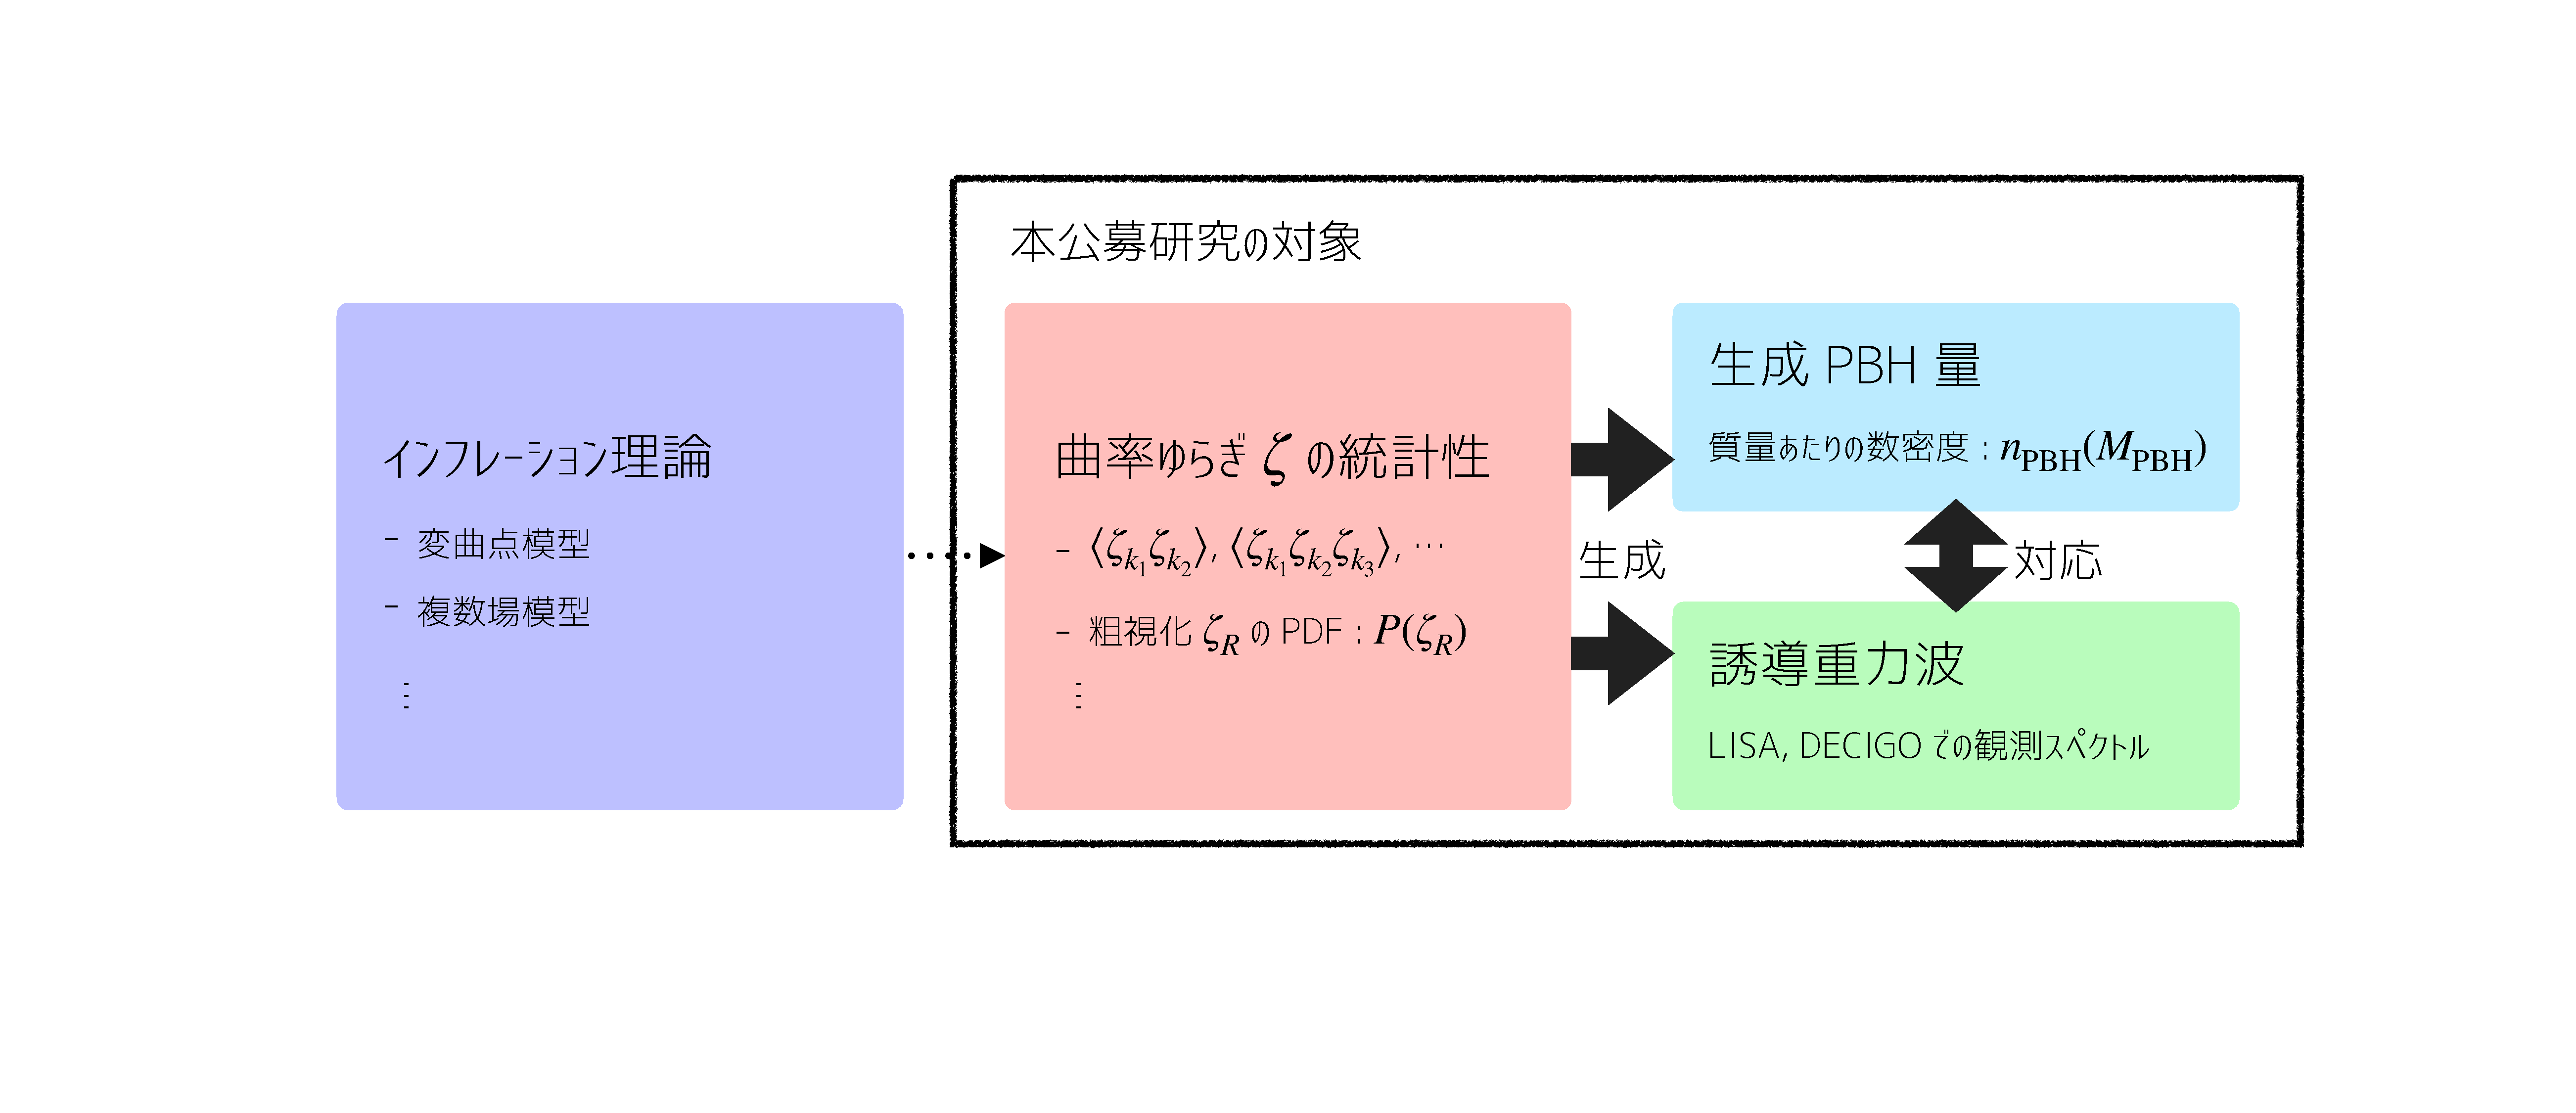
\includegraphics[width=\hsize]{figs/abstract.pdf}
	\caption{本研究対象の相関図. 宇宙初期の加速膨張であるインフレーションによって様々な天体のもととなる曲率ゆらぎが生成される. 大きな曲率ゆらぎはダークマターの候補となる PBH だけでなく,
	背景重力波も誘導生成する. 誘導重力波の生成量には大きな不定性はないが, PBH の生成量の見積もりは未だ正確には定式化されていない. 本研究では曲率ゆらぎから PBH 生成量の見積もりを定式化することで,
	曲率ゆらぎを介し PBH 量と誘導重力波量を正確に対応づけることを目的とする.}
	\label{fig: abstract}
\end{figure}
	
%\vspace*{10zw}	% (概要)と(本文)の間が10行程度になるよう、必要に応じて値を調整してください。	
%end 研究目的及び研究計画の概要空行付き ====================

%\noindent
%\rule{\linewidth}{1pt}\\
\newpage
\noindent
\textbf{(本文)}
%begin 研究目的と研究計画	====================

\begin{mdframed}[roundcorner=0.5zw,
	%skipabove=1zw,skipbelow=1zw,
	innertopmargin=0.8zw,innerbottommargin=0.8zw,
	%innerleftmargin=0.8zw,innerrightmargin=0.8zw,
	%rightmargin=5000pt,leftmargin=50pt,
	linecolor=black!50,linewidth=0.2zw,
	backgroundcolor=black!10]
	{\bfseries\gtfamily\sffamily\large 1. 研究の学術的背景および核心となる「問い」}
\end{mdframed}

\noindent
ダークマターは存在が確実視されているものの, その正体は未だ解明されていない.
これまでその候補として WIMP (Weakly Interacting Massive Particle) が注目されてきたが, 様々な観測および実験から制限が厳しくなっているのが現状である.
そこで本領域研究では WIMP に捉われない, 多角的なダークマター探索を目的としている.
その中の1つが\emph{原始ブラックホール (Primordial Black Hole: PBH)} に代表される巨視的ダークマターであり,
本公募研究においてもダークマターとしての PBH を主対象とする.

そもそも宇宙における銀河などの豊かな構造は, インフレーションと呼ばれる宇宙初期の加速膨張期に作られた空間曲率のゆらぎ ($\zeta$ と書かれる) をもとにしていると考えられている.
この曲率ゆらぎは大規模 ($\gtrsim1\,\mathrm{Mpc}$) では非常に小さい ($\zeta\sim10^{-5}$) ことが宇宙マイクロ波背景放射 (Cosmic Microwave Background: CMB) の観測などから知られているが~\cite{Aghanim:2018eyx},
小規模でも小さいかどうかはわかっていない.
もし小規模では大きな曲率ゆらぎがありふれていて, $\zeta\sim1$ となるような領域が無視できない確率で生じたとすると, その領域は宇宙初期の放射優勢期に星を介さず直接ブラックホールまで重力崩壊することが予想されており,
このようなブラックホールを PBH と呼ぶ~\cite{Carr:1974nx}.
通常のブラックホールは重い星の超新星爆発から生じるため典型的に太陽質量 $M_\odot$ 程度にしかならないのに対し,
PBH は星を介さないためほぼ任意の質量で実現できることが大きな特徴である.
例えば非常に重い PBH ($\gtrsim10^4M_\odot$) は各銀河中心に存在する (そして近年 Event Horizon Telescope で撮像に成功した) 超大質量ブラックホールの種天体の候補の1つであるし~\cite{Carr:2018rid},
LIGO/Virgo で合体重力波を通して観測されたやや重いブラックホール ($\sim10M_\odot$) も PBH である可能性が指摘されている~\cite{Sasaki:2018dmp}.

ブラックホールは基本的に重力的にしか相互作用しないため, 十分な PBH 量があればダークマターとしても振る舞うことができる.
現在までに様々な質量の PBH に対し多様な観測的制限がかけられてきたが, $\sim(10^{-15}\text{--}10^{-11})M_\odot$ 程度の小惑星のように軽い PBH に対しては確かな制限はかかっておらず, ダークマターの主成分になり得るため注目されている~\cite{Carr:2016drx}.
しかしそれは逆に言えば, \ul{このような PBH がダークマターの主成分であったとしてもそれを観測的に確かめる手段は未だ確立されていない}ことを意味する.
本領域研究でも様々な観測手段によって PBH を捉える研究が行われるが,
本公募研究でも\emph{「小惑星型 PBH がダークマターであるときそれを検証する手段はあるか?」}という問いを核心に据える.




\begin{mdframed}[roundcorner=0.5zw,
	%skipabove=1zw,skipbelow=1zw,
	innertopmargin=0.8zw,innerbottommargin=0.8zw,
	%innerleftmargin=0.8zw,innerrightmargin=0.8zw,
	%rightmargin=5000pt,leftmargin=50pt,
	linecolor=black!50,linewidth=0.2zw,
	backgroundcolor=black!10]
	{\bfseries\gtfamily\sffamily\large 2. 研究の目的および学術的独自性}
\end{mdframed}

\noindent
小惑星型 PBH に限らず多くの質量帯において PBH の相補的根拠として期待されているのが重力波である.
PBH を作るほど大きな曲率ゆらぎがありふれていた場合, PBH ができなかった領域 ($\zeta\sim10^{-2}$程度) でも曲率ゆらぎどうしの相互作用から十分な大きさの\emph{背景重力波が誘導}されることが指摘されている~\cite{Saito:2008jc}.
誘導重力波の周波数は曲率ゆらぎの相関長, すなわち生成される PBH 質量と対応しており, 
例えば LIGO/Virgo 重力波に関係する $\calO(10)M_\odot$ PBH に対応する周波数は $\sim1\mathrm{nHz}$ 程度で,
パルサーの同期観測 (Pulsar Timing Array: PTA) によって測定することができる.
近年 PTA 観測の1つである NANOGrav グループが実際に背景重力波を観測した可能性を報告し~\cite{Arzoumanian:2020vkk},
PBH に対応する誘導重力波の現実的な観測可能性が高まっている.

小惑星型 PBH に対応する周波数は $\sim1\mathrm{mHz}$ 程度であり,
ちょうど LISA や DECIGO 計画に代表される衛星型重力波望遠鏡の周波数帯である.
すなわち\ul{小惑星型 PBH がダークマターであった場合 LISA や DECIGO で誘導重力波が観測される}ことが期待され, 
小惑星型 PBH ダークマターの観測的根拠となり得る.
このような学術背景から今こそ PBH と誘導重力波の関係を精査する必要があると言える.

PBH 量と誘導重力波量を正確に対応づけるためには, その両方のもととなる曲率ゆらぎの統計的性質との対応を精査しなければならない.
これまで曲率ゆらぎは基本的にガウス分布に従うと仮定され, 非ガウス性の補正は級数展開によってしばしば取り入れられてきた~\cite{Byrnes:2012yx}.
例えば曲率ゆらぎ $\zeta$ はガウス場 $g$ を用い, 以下のような展開によって近似される.
\bae{\label{eq: fNL expansion}
	\zeta(\bfx)=g(\bfx)+\frac{3}{5}\fNL g^2(\bfx)+\cdots.
}
展開係数 $\fNL$ は非線形パラメータと呼ばれ, 数値因子 $3/5$ は慣習である.
誘導重力波に対し重要になる曲率ゆらぎの大きさは $\zeta\sim10^{-2}$, すなわち $g\sim10^{-2}$ 程度であり, $1$より十分小さいのでこのような展開近似は正当化される.
しかしながら PBH には $\zeta\sim1$ のゆらぎが必要であり, このような領域に対し上記の展開は全く適当ではない.
実際具体的なインフレーション理論において\ul{曲率ゆらぎは大きい部分でガウス分布 ({$\propto\exp(-\zeta^2)$}) ではなく
指数関数 ({$\propto\exp(-\zeta)$}) でしか減衰しない}可能性が指摘されている~\cite{Ezquiaga:2019ftu}.
さらに仮に曲率ゆらぎの統計が正確に指定されたとしても, そこから PBH 量を見積もる段階では Press-Schechter と呼ばれる簡単化された統計手法が使われることが多かった.
Press-Schechter 法では空間的に粗視化した曲率ゆらぎが, ある閾値を超えるか否かのみで PBH 形成が判定されるが,
実際の PBH 形成は曲率ゆらぎの配位形にも依存するため, 本来は配位形を決める特徴量も全て統計的に扱わなければならない.
これらを踏まえ本公募研究では\emph{「任意の曲率ゆらぎ統計に対し Press-Schechter を超えた正確な統計処理により PBH 量を見積もる」}ことを目的とする.


\begin{mdframed}[roundcorner=0.5zw,
	%skipabove=1zw,skipbelow=1zw,
	innertopmargin=0.8zw,innerbottommargin=0.8zw,
	%innerleftmargin=0.8zw,innerrightmargin=0.8zw,
	%rightmargin=5000pt,leftmargin=50pt,
	linecolor=black!50,linewidth=0.2zw,
	backgroundcolor=black!10]
	{\bfseries\gtfamily\sffamily\large 3. 研究の具体的計画}
\end{mdframed}

\noindent
Press-Schechter 法を超えた PBH 量の見積もりとして, 近年本領域研究の A03 理論班研究代表者である\emph{柳哲文氏 (名古屋大講師)} らにより,
乱数場の平均値周りの統計ではなく「極端に大きな値」の統計を扱う\emph{ピーク理論}を PBH に応用した研究が発表された~\cite{Yoo:2018kvb}.
ピーク理論によれば極端に大きな値 (ピーク) の配位形は球対称に近くなり, 「値の大きさ」と「配位の相関長」の2変数のみで記述できることがわかる.
これら2変数の確率分布はもとの曲率ゆらぎの統計性から決定される.
一方球対称配位での PBH 形成条件は解析的にも数値的にも研究され, 「圧縮率」という特徴量で良く判定できることが知られている.
したがって「圧縮率」を「値の大きさ」と「配位の相関長」の2変数関数として与えておけば, 
PBH 形成確率を正確に議論することができるということが明らかにされた.

本論文ではまずもとの曲率ゆらぎがガウス場で, かつ特定の相関長しか持たない場合 (単色スペクトルと呼ぶ) についてのみ議論された.
続いて\emph{横山修一郎氏 (名古屋大助教)} らとともに, 非ガウス補正として \eqref{eq: fNL expansion}~式の2次項 ($\fNL$) を加え (しかし単色スペクトルのまま) 議論が拡張された~\cite{Yoo:2019pma}.
それとは独立に柳氏らにより, ガウス場のまましかし任意スペクトルに対しての拡張も行われている~\cite{Yoo:2020dkz}.
そこで現在申請者は柳・横山両氏, さらに\emph{北嶋直弥 (東北大助教)} の協力のもと, 両研究を統合し\emph{\boldmath「任意スペクトルかつ $\fNL$ 補正まで入った PBH ピーク理論の構築」}を議論し始めている.
この研究の完成が\ul{第一の研究計画}である.

一方上述した通り PBH 形成を左右するような大きな曲率ゆらぎに対し $\fNL$ 級数展開は正当化されない.
実際具体的なインフレーション理論において大きな曲率ゆらぎの統計性はガウス分布から著しくずれる可能性がある.
そこで\ul{第二の研究計画}は\emph{「任意スペクトルかつ実際のインフレーション理論に示唆される非ガウス分布に対する PBH ピーク理論の構築」}とする.
ここで「インフレーション理論に示唆される曲率ゆらぎの統計性」は実は申請者がこれまで研究してきた「インフレーションの確率形式」と呼ばれる解析手法 (3 応募者の研究遂行能力及び研究環境も参照) で計算されることに触れておく.
したがって申請者は具体的な曲率ゆらぎの統計性の導出にも精通しており, この具体形を参考に PBH ピーク理論を構築する.
ガウス分布を仮定しない場合, ピークの「値の大きさ」と「配位の相関長」の確率分布は解析的には解けないかもしれないが,
少なくとも数値的には解けることが期待される.
これらの解析的あるいは数値的研究に計算機ソフトウェア \textsc{Mathematica} を利用するため,
その費用が本研究費の使途の1つである.




\begin{mdframed}[roundcorner=0.5zw,
	%skipabove=1zw,skipbelow=1zw,
	innertopmargin=0.8zw,innerbottommargin=0.8zw,
	%innerleftmargin=0.8zw,innerrightmargin=0.8zw,
	%rightmargin=5000pt,leftmargin=50pt,
	linecolor=black!50,linewidth=0.2zw,
	backgroundcolor=black!10]
	{\bfseries\gtfamily\sffamily\large 4. 当該研究領域の推進への貢献}
\end{mdframed}

\noindent
本領域研究ではダークマターの探索を目的としており, 3つの大きな目標のうちの1つが PBH に代表される巨視的ダークマターである.
これまで申請者は PBH ダークマターを実現するインフレーション理論の提唱などの観点から貢献してきたが (3 応募者の研究遂行能力及び研究環境も参照),
PBH がダークマターであることを裏付けるためには相補的な観測根拠が不可欠である.
誘導重力波はその有力な候補の1つであり, 様々な重力波観測計画が実現しようとしている現在において,
重力波量と PBH 量を正確に対応づける研究は必須である.
この研究を通じ, もし重力波が観測されて PBH の存在量と質量が正確に判明すれば, 
他の様々な観測的検証 (本領域研究でも計画されている重力レンズや蒸発光など) の助けになり,
逆にこれらの観測で先に PBH が発見され, 対応する誘導重力波量が予想されれば, 重力波観測計画の促進につながるであろう.

これらが本公募研究の当該研究領域の推進への貢献であり, 以上が具体的な研究目的および研究方法である.



\bigskip

\begin{thebibliography}{99}

\scriptsize % フォントサイズを下げる
\setlength{\itemsep}{-2pt} % 行間を縮める

%\cite{Aghanim:2018eyx}
\bibitem{Aghanim:2018eyx}
N.~Aghanim \textit{et al.} [Planck],
%``Planck 2018 results. VI. Cosmological parameters,''
Astron. Astrophys. \textbf{641}, A6 (2020)
%doi:10.1051/0004-6361/201833910
[arXiv:1807.06209 [astro-ph.CO]].
%4684 citations counted in INSPIRE as of 23 Mar 2021

%\cite{Carr:1974nx}
\bibitem{Carr:1974nx}
B.~J.~Carr and S.~W.~Hawking,
%``Black holes in the early Universe,''
Mon. Not. Roy. Astron. Soc. \textbf{168}, 399-415 (1974)
%818 citations counted in INSPIRE as of 23 Mar 2021

%\cite{Carr:2018rid}
\bibitem{Carr:2018rid}
B.~Carr and J.~Silk,
%``Primordial Black Holes as Generators of Cosmic Structures,''
Mon. Not. Roy. Astron. Soc. \textbf{478}, no.3, 3756-3775 (2018)
%doi:10.1093/mnras/sty1204
[arXiv:1801.00672 [astro-ph.CO]].
%89 citations counted in INSPIRE as of 24 Mar 2021

%\cite{Sasaki:2018dmp}
\bibitem{Sasaki:2018dmp}
M.~Sasaki, T.~Suyama, T.~Tanaka and S.~Yokoyama,
%``Primordial black holes\textemdash{}perspectives in gravitational wave astronomy,''
Class. Quant. Grav. \textbf{35}, no.6, 063001 (2018)
%doi:10.1088/1361-6382/aaa7b4
[arXiv:1801.05235 [astro-ph.CO]].
%284 citations counted in INSPIRE as of 24 Mar 2021

%\cite{Carr:2016drx}
\bibitem{Carr:2016drx}
B.~Carr, F.~Kuhnel and M.~Sandstad,
%``Primordial Black Holes as Dark Matter,''
Phys. Rev. D \textbf{94}, no.8, 083504 (2016)
%doi:10.1103/PhysRevD.94.083504
[arXiv:1607.06077 [astro-ph.CO]].
%599 citations counted in INSPIRE as of 24 Mar 2021

%\cite{Saito:2008jc}
\bibitem{Saito:2008jc}
R.~Saito and J.~Yokoyama,
%``Gravitational wave background as a probe of the primordial black hole abundance,''
Phys. Rev. Lett. \textbf{102}, 161101 (2009)
[erratum: Phys. Rev. Lett. \textbf{107}, 069901 (2011)]
%doi:10.1103/PhysRevLett.102.161101
[arXiv:0812.4339 [astro-ph]].
%156 citations counted in INSPIRE as of 24 Mar 2021

%\cite{Arzoumanian:2020vkk}
\bibitem{Arzoumanian:2020vkk}
Z.~Arzoumanian \textit{et al.} [NANOGrav],
%``The NANOGrav 12.5 yr Data Set: Search for an Isotropic Stochastic Gravitational-wave Background,''
Astrophys. J. Lett. \textbf{905}, no.2, L34 (2020)
%doi:10.3847/2041-8213/abd401
[arXiv:2009.04496 [astro-ph.HE]].
%104 citations counted in INSPIRE as of 24 Mar 2021

%\cite{Byrnes:2012yx}
\bibitem{Byrnes:2012yx}
C.~T.~Byrnes, E.~J.~Copeland and A.~M.~Green,
%``Primordial black holes as a tool for constraining non-Gaussianity,''
Phys. Rev. D \textbf{86}, 043512 (2012)
%doi:10.1103/PhysRevD.86.043512
[arXiv:1206.4188 [astro-ph.CO]].
%89 citations counted in INSPIRE as of 24 Mar 2021

%\cite{Ezquiaga:2019ftu}
\bibitem{Ezquiaga:2019ftu}
J.~M.~Ezquiaga, J.~Garc\'\i{}a-Bellido and V.~Vennin,
%``The exponential tail of inflationary fluctuations: consequences for primordial black holes,''
JCAP \textbf{03}, 029 (2020)
%doi:10.1088/1475-7516/2020/03/029
[arXiv:1912.05399 [astro-ph.CO]].
%25 citations counted in INSPIRE as of 24 Mar 2021

%\cite{Yoo:2018kvb}
\bibitem{Yoo:2018kvb}
C.~M.~Yoo, T.~Harada, J.~Garriga and K.~Kohri,
%``Primordial black hole abundance from random Gaussian curvature perturbations and a local density threshold,''
PTEP \textbf{2018}, no.12, 123E01 (2018)
%doi:10.1093/ptep/pty120
[arXiv:1805.03946 [astro-ph.CO]].
%75 citations counted in INSPIRE as of 24 Mar 2021

%\cite{Yoo:2019pma}
\bibitem{Yoo:2019pma}
C.~M.~Yoo, J.~O.~Gong and S.~Yokoyama,
%``Abundance of primordial black holes with local non-Gaussianity in peak theory,''
JCAP \textbf{09}, 033 (2019)
%doi:10.1088/1475-7516/2019/09/033
[arXiv:1906.06790 [astro-ph.CO]].
%23 citations counted in INSPIRE as of 24 Mar 2021

%\cite{Yoo:2020dkz}
\bibitem{Yoo:2020dkz}
C.~M.~Yoo, T.~Harada, S.~Hirano and K.~Kohri,
%``Abundance of Primordial Black Holes in Peak Theory for an Arbitrary Power Spectrum,''
PTEP \textbf{2021}, no.1, 013E02 (2021)
%doi:10.1093/ptep/ptaa155
[arXiv:2008.02425 [astro-ph.CO]].
%9 citations counted in INSPIRE as of 24 Mar 2021


\end{thebibliography}

%end 研究目的と研究計画	====================

% p01_purpose_plan_01.tex
\KLEndSubject{F}


%#Split: 02_background  
%#PieceName: p02_background
% p02_background_00.tex
\KLBeginSubject{02}{2}{2 本研究の着想に至った経緯など}{1}{F}{}{jsps-subject-header}{jsps-default-header}

\section{2 本研究の着想に至った経緯など}
%    <<最大 1ページ>>

%s03_background
%begin 本研究の着想に至った経緯など ====================

\begin{mdframed}[roundcorner=0.5zw,
	%skipabove=1zw,skipbelow=1zw,
	innertopmargin=0.8zw,innerbottommargin=0.8zw,
	%innerleftmargin=0.8zw,innerrightmargin=0.8zw,
	%rightmargin=5000pt,leftmargin=50pt,
	linecolor=black!50,linewidth=0.2zw,
	backgroundcolor=black!10]
	{\bfseries\gtfamily\sffamily\large 1. 着想に至った経緯と準備状況}
\end{mdframed}

\noindent
PBH 形成は一般相対論の非線形効果によって起こるため, その判定は難しい.
近年になるまでは「PBH を実現できるか否か」のみが主に注目され, PBH 量自体はインフレーション理論のパラメータを少し変え, 曲率ゆらぎの統計性をわずかに変化させるだけでいくらでも調整できるため,
あまり正確に議論されては来なかった.
しかし PBH 形成に誘導重力波が伴うこと, そして重力波観測が現実味を帯びてきた現状を踏まえ, PBH の相補的根拠として誘導重力波を用いることが真剣に捉えられるようになってきた.
誘導重力波を PBH の相補的根拠とするには, もととなる曲率ゆらぎの統計性を固定し, PBH と誘導重力波双方の生成量を正確に見積もらなければならない.
したがって \ul{PBH 量の正確な議論の需要}が高まっているのが現状である.

一方ブラックホール形成の解析的および数値的研究の進歩により, 様々なピーク配位に対する PBH 形成判定が議論できるようになってきた.
さらに申請者がこれまで推し進めてきた「インフレーションの確率形式」の発展により, インフレーションによって作られる曲率ゆらぎに対し, ピーク付近での統計性が計算できるようになってきている.
すなわち \ul{PBH 量の正確な議論の供給}も可能になっていると言える.

申請者はこれまでインフレーションの確率形式の研究を通じ, 曲率ゆらぎのピーク付近の統計がガウス分布からずれ得ることを知り,
また自身の論文 (3-[\ref{ref: PBH tower}, \ref{ref: PBH bias}]) でも議論したように, 曲率ゆらぎの非ガウス性や PBH 形成判定条件が PBH 量に大きな影響を与えることを考察してきた.
このような経験と, 上述した PBH 量の正確な議論の需要と供給の一致が本研究計画の着想に至った経緯である.

準備状況としては 1-3 で触れた通り現在, 柳, 横山, 北嶋氏の協力のもと「任意スペクトルかつ $\fNL$ 補正まで入った PBH ピーク理論の構築」を進めている.
理論のアルゴリズム自体の構築には成功しており, 様々なスペクトル形に対し具体的な計算を行なっている最中である.
また現状アルゴリズム自体は完成していてもその具体計算には複雑な数値計算が必要になっており, 今後の発展や多くの研究者にとっての利用しやすさのためにも,
各段階における解析的整備を行えないか検討中である.


\begin{mdframed}[roundcorner=0.5zw,
	%skipabove=1zw,skipbelow=1zw,
	innertopmargin=0.8zw,innerbottommargin=0.8zw,
	%innerleftmargin=0.8zw,innerrightmargin=0.8zw,
	%rightmargin=5000pt,leftmargin=50pt,
	linecolor=black!50,linewidth=0.2zw,
	backgroundcolor=black!10]
	{\bfseries\gtfamily\sffamily\large 2. 本研究の世界的位置付け}
\end{mdframed}

\noindent
PBH 形成判定条件の研究は柳氏らのグループに限らず現在世界的に注目されている (論文~\cite{Escriva:2019phb} 等).
それら条件を用いて PBH 量を推定する統計手法も乱立している (論文~\cite{DeLuca:2020ioi,Young:2020xmk} 等).
一方で曲率ゆらぎピークの統計がガウス分布から大きくずれ得ることも認知されてきている (論文~1-\cite{Ezquiaga:2019ftu}や\cite{Figueroa:2020jkf}).
これらはまだそれぞれ独立した研究であり, したがって本研究は\ul{これらを1つにまとめ上げる}研究であると言える.
PBH を観測的に立証するには誘導重力波の立ち位置は重く, 本研究はその理論的整備を行うだけでなく,
他の PBH 直接観測計画や重力波観測計画の推進にも貢献するであろう.

\bigskip

\begin{thebibliography}{99}

\scriptsize % フォントサイズを下げる
\setlength{\itemsep}{-2pt} % 行間を縮める

%\cite{Escriva:2019phb}
\bibitem{Escriva:2019phb}
A.~Escriv\`a, C.~Germani and R.~K.~Sheth,
%``Universal threshold for primordial black hole formation,''
Phys. Rev. D \textbf{101}, no.4, 044022 (2020)
%doi:10.1103/PhysRevD.101.044022
[arXiv:1907.13311 [gr-qc]].
%49 citations counted in INSPIRE as of 24 Mar 2021

%\cite{DeLuca:2020ioi}
\bibitem{DeLuca:2020ioi}
V.~De Luca, G.~Franciolini and A.~Riotto,
%``On the Primordial Black Hole Mass Function for Broad Spectra,''
Phys. Lett. B \textbf{807}, 135550 (2020)
%doi:10.1016/j.physletb.2020.135550
[arXiv:2001.04371 [astro-ph.CO]].
%15 citations counted in INSPIRE as of 24 Mar 2021

%\cite{Young:2020xmk}
\bibitem{Young:2020xmk}
S.~Young and M.~Musso,
%``Application of peaks theory to the abundance of primordial black holes,''
JCAP \textbf{11}, 022 (2020)
%doi:10.1088/1475-7516/2020/11/022
[arXiv:2001.06469 [astro-ph.CO]].
%8 citations counted in INSPIRE as of 24 Mar 2021

%\cite{Figueroa:2020jkf}
\bibitem{Figueroa:2020jkf}
D.~G.~Figueroa, S.~Raatikainen, S.~Rasanen and E.~Tomberg,
%``Non-Gaussian tail of the curvature perturbation in stochastic ultra-slow-roll inflation: implications for primordial black hole production,''
[arXiv:2012.06551 [astro-ph.CO]].
%1 citations counted in INSPIRE as of 24 Mar 2021

\end{thebibliography}


%end 本研究の着想に至った経緯など ====================

% p02_background_01.tex
\KLEndSubject{F}


%#Split: 03_abilities  
%#PieceName: p03_abilities
% p03_abilities_00.tex
\KLBeginSubject{03}{3}{3 応募者の研究遂行能力及び研究環境}{2}{F}{}{jsps-subject-header}{jsps-default-header}

\section{3 応募者の研究遂行能力及び研究環境}
%    <<最大 2ページ>>

% s14_abilities
%begin 応募者の研究遂行能力及び研究環境 ====================

\begin{mdframed}[roundcorner=0.5zw,
	%skipabove=1zw,skipbelow=1zw,
	innertopmargin=0.8zw,innerbottommargin=0.8zw,
	%innerleftmargin=0.8zw,innerrightmargin=0.8zw,
	%rightmargin=5000pt,leftmargin=50pt,
	linecolor=black!50,linewidth=0.2zw,
	backgroundcolor=black!10]
	{\bfseries\gtfamily\sffamily\large 1. これまでの研究活動}
\end{mdframed}

\noindent
申請者のこれまでの経歴や業績を以下に簡単にまとめた. 
申請者の web ページ \url{https://nekomammat.github.io/indexJP.html} も合わせて参照されたい.

\begin{description}\itemsep-1mm \itemindent4zw \labelwidth6zw
	\item[\gtfamily 学術論文 計22報 (以下代表作)]
\end{description}
\vspace{-7mm}
\begin{enumerate}\itemsep-2mm
	\item K.~T.~Abe, \underline{Y.~Tada} and I.~Ueda,
	``Induced gravitational waves as a cosmological probe of the sound speed during the QCD phase transition,''
	[arXiv:2010.06193 [astro-ph.CO]].
	\label{ref: GW QCD}

	\item L.~Pinol, S.~Renaux-Petel and \underline{Y.~Tada},
	``A manifestly covariant theory of multifield stochastic inflation in phase space,''
	JCAP accepted [arXiv:2008.07497 [astro-ph.CO]].
	\label{ref: manifestly covariant}
	
	\item Y.~Mikura, \underline{Y.~Tada} and S.~Yokoyama, 
	``Conformal inflation in the metric-affine geometry,''
	EPL \textbf{132}, no.3, 39001 (2020) 
	[arXiv:2008.00628 [hep-th]], 
	\emph{Editor's Choice}. 
	\label{ref: conformal inflation}
	
	\item \underline{Y.~Tada} and S.~Yokoyama,
	``Primordial black hole tower: Dark matter, earth-mass, and LIGO black holes,''
	Phys. Rev. D \textbf{100}, no.2, 023537 (2019)
	[arXiv:1904.10298 [astro-ph.CO]].
	\label{ref: PBH tower}
	
	\item L.~Pinol, S.~Renaux-Petel and \underline{Y.~Tada}, ``Inflationary stochastic anomalies,''
	Class. Quant. Grav. \textbf{36}, no.7, 07LT01 (2019)
	[arXiv:1806.10126 [gr-qc]],
	\emph{Highlights of 2019--20}.
	\label{ref: stochastic anomaly}
	
	\item K.~Inomata, M.~Kawasaki, K.~Mukaida, \underline{Y.~Tada} and T.~T.~Yanagida,
	``$\mathcal O(10) M_\odot$ primordial black holes and string axion dark matter,''
	Phys. Rev. D \textbf{96}, no.12, 123527 (2017)
	[arXiv:1709.07865 [astro-ph.CO]].
	\label{ref: O(10) PBH}
	
	\item K.~Inomata, M.~Kawasaki, K.~Mukaida, \underline{Y.~Tada} and T.~T.~Yanagida,
	``Inflationary Primordial Black Holes as All Dark Matter,''
	Phys. Rev. D \textbf{96}, no.4, 043504 (2017)
	[arXiv:1701.02544 [astro-ph.CO]].
	\label{ref: PBH DM}

	\item K.~Inomata, M.~Kawasaki, K.~Mukaida, \underline{Y.~Tada} and T.~T.~Yanagida,
	``Inflationary primordial black holes for the LIGO gravitational wave events and pulsar timing array experiments,''
	Phys. Rev. D \textbf{95}, no.12, 123510 (2017)
	[arXiv:1611.06130 [astro-ph.CO]].
	\label{ref: PBH LIGO}
	
	\item M.~Kawasaki, A.~Kusenko, \underline{Y.~Tada} and T.~T.~Yanagida,
	``Primordial black holes as dark matter in supergravity inflation models,''
	Phys. Rev. D \textbf{94}, no.8, 083523 (2016)
	[arXiv:1606.07631 [astro-ph.CO]].
	\label{ref: PBH SUGRA}

	\item M.~Kawasaki and \underline{Y.~Tada},
	``Can massive primordial black holes be produced in mild waterfall hybrid inflation?,''
	JCAP \textbf{08}, 041 (2016)
	[arXiv:1512.03515 [astro-ph.CO]].
	\label{ref: PBH hybrid}
	
	\item \underline{Y.~Tada} and S.~Yokoyama,
	``Primordial black holes as biased tracers,''
	Phys. Rev. D \textbf{91}, no.12, 123534 (2015)
	[arXiv:1502.01124 [astro-ph.CO]].
	\label{ref: PBH bias}

	\item T.~Fujita, M.~Kawasaki and \underline{Y.~Tada},
	``Non-perturbative approach for curvature perturbations in stochastic $\delta N$ formalism,''
	JCAP \textbf{10}, 030 (2014)
	[arXiv:1405.2187 [astro-ph.CO]].
	\label{ref: stochastic hybrid}

	\item T.~Fujita, M.~Kawasaki, \underline{Y.~Tada} and T.~Takesako,
	``A new algorithm for calculating the curvature perturbations in stochastic inflation,''
	JCAP \textbf{12}, 036 (2013)
	[arXiv:1308.4754 [astro-ph.CO]].
	\label{ref: stochastic-dN}
			
\end{enumerate}
\begin{description}\itemsep-1mm \itemindent4zw \labelwidth6zw
	\item[\gtfamily 職歴・フェローシップ]
	\item[\rm\sffamily 2021.04--] \emph{特任助教} 名古屋大学 高等研究院, 理学研究科 宇宙論研究室 (着任予定)
	\item[\rm\sffamily 2019.04--] \emph{非常勤講師 (力学1, 2)} 大同大学
	\item[\rm\sffamily 2018.04--] \emph{日本学術振興会特別研究員 PD} 名古屋大学大学院 理学研究科 宇宙論研究室
	\item[\rm\sffamily 2017.04--] \emph{ポスドク研究員} \itemsep-2mm
	\item[\rm\sffamily\hfill 2018.03  ] Institut d'Astrophysique de Paris, France \itemsep-1mm
	\item[\rm\sffamily 2015.04--] \emph{日本学術振興会特別研究員 DC2} \itemsep-2mm
	\item[\rm\sffamily\hfill 2017.03  ] 東京大学 カブリ数物連携宇宙研究機構および宇宙線研究所 \itemsep-1mm
	\item[\rm\sffamily 2012.10--] \emph{フォトンサイエンス・リーディング大学院} \itemsep-2mm
	\item[\rm\sffamily\hfill 2017.03  ] 東京大学 カブリ数物連携宇宙研究機構および宇宙線研究所
\end{description}
\begin{description}\itemsep-1mm \itemindent4zw \labelwidth6zw
	\item[\gtfamily 採択・受賞歴]
	\item[\rm\sffamily 2020.11.27] \emph{Outstanding Presentation Award Gold Prize} Online JGRG Workshop 2020
	\item[\rm\sffamily 2019.02] \emph{若手代表発表者} FAPESP-JSPS Workshop on dark energy, dark matter, and galaxies
	\item[\rm\sffamily 2017.02.24] \emph{所長賞 (博士部門)} 第6回修士博士研究発表会, 宇宙線研究所
\end{description}
\begin{description}\itemsep-1mm \itemindent4zw \labelwidth6zw
	\item[\gtfamily 外部資金獲得状況]
	\item[\rm\sffamily 2019--2020] \emph{科学研究費助成事業 若手研究} \\
		JP19K14707「ストカスティック形式で迫る重力と量子論」1,560,000 円, 研究代表者
\end{description}
\begin{description}\itemsep-1mm \itemindent4zw \labelwidth6zw
	\item[\gtfamily 研究者活動]
	\item[\hfill -] \emph{研究発表} \itemsep-2mm
	\item[] 国際会議 計26件, 国内会議 計12件, セミナー発表 国内外計24件 \itemsep-1mm
	\item[\hfill -] \emph{サイエンスメンバー} \itemsep-2mm
	\item[] International Research Network Extragalactic astrophysics and Cosmology (NECO) \itemsep-1mm
	\item[\hfill -] \emph{査読} EPJC, JCAP, MPLA, PRD, PTEP, Universe
	\item[\rm\sffamily 2014.10.01--] \emph{留学} ヘルシンキ大学 Kari Enqvist 教授 \itemsep-2mm
	\item[\rm\sffamily\hfill 12.22  ] フォトンサイエンス・リーディング大学院のコースワーク \itemsep-1mm
\end{description}

\noindent
申請者はこれまで\ul{原始ブラックホール (PBH)} と\ul{インフレーションの確率形式}について, 本研究課題に密接に関連した研究を重点的に行ってきた.
PBH に関しては論文~[\ref{ref: PBH tower}, \ref{ref: O(10) PBH}--\ref{ref: PBH bias}] を発表,
特に論文~[\ref{ref: PBH DM}, \ref{ref: PBH SUGRA}] ではダークマターとして, 論文~[\ref{ref: PBH LIGO}] では LIGO 重力波の波源として,
そして論文~[\ref{ref: PBH tower}] ではそれら観測的動機を同時に説明する天体としての PBH 形成を議論している.
論文~[\ref{ref: PBH LIGO}] では誘導重力波が PBH の検証に重要であることを再指摘し, 論文~[\ref{ref: PBH tower}] では PBH 質量と観測的動機, 誘導重力波の周波数, および
対応する重力波観測計画を改めて明確にした.
論文~[\ref{ref: GW QCD}] ではさらに誘導重力波を宇宙の量子色力学相転移の検証への応用を議論している.

一方, 乱数を扱う数学である\emph{確率形式}をインフレーションに応用し, 曲率ゆらぎを非摂動的に計算する手法を提唱~[\ref{ref: stochastic hybrid}, \ref{ref: stochastic-dN}], 
PBH を実現するような大きなゆらぎも扱える可能性を提示した.
論文~[\ref{ref: PBH hybrid}] では実際に特定のインフレーション理論に確率形式を適用し PBH 形成を議論した.
フランスでは本確率形式をインフレーション理論の一般形に適用できるよう, インフレーションの確率形式を一から数学的に定式化し直した~[\ref{ref: manifestly covariant}, \ref{ref: stochastic anomaly}].
以上のように申請者はこれまで\ul{当該領域で十分な実績を挙げており, 本研究課題の遂行可能性を客観的に示している}.


\begin{mdframed}[roundcorner=0.5zw,
	%skipabove=1zw,skipbelow=1zw,
	innertopmargin=0.8zw,innerbottommargin=0.8zw,
	%innerleftmargin=0.8zw,innerrightmargin=0.8zw,
	%rightmargin=5000pt,leftmargin=50pt,
	linecolor=black!50,linewidth=0.2zw,
	backgroundcolor=black!10]
	{\bfseries\gtfamily\sffamily\large 2. 研究環境}
\end{mdframed}

\noindent
名古屋大学高等研究院の特任助教に内定を得たため, 引き続き名古屋大学宇宙論研究室で安定した研究活動が可能である.
当研究室において PBH や誘導重力波に関する共同研究実績を挙げており~[\ref{ref: GW QCD}, \ref{ref: PBH tower}] (論文~[\ref{ref: conformal inflation}] も大学院生の教育実績として参照されたい),
本研究課題に対して研究環境が適していることを示している.
特に PBH に関しては A03 理論班の研究代表者である\emph{柳哲文氏 (名古屋大講師)} や PBH 研究の第一人者の一人である\emph{横山修一郎氏 (名古屋大助教)}の協力を仰げる, 
非常に優れた研究環境だと言える.
他には重力波計算に精通した\emph{北嶋直弥氏 (東北大助教)}とも共同で研究を行う.
設備面では, 確率解析や統計の数値計算は並列化と相性が良く, コア数の多い PC や計算ツール (Mathematica) が必要である.
これら共同研究のための旅費や設備準備費として本科学研究費が不可欠である.


	
%end 応募者の研究遂行能力及び研究環境 ====================
%begin 研究業績リスト ====================
	
	%end 研究業績リスト ====================

% p03_abilities_01.tex
\KLEndSubject{F}


%#Split: 04_rights  
%#PieceName: p04_rights
% p04_rights_00.tex
\KLBeginSubject{04}{4}{4 人権の保護及び法令等の遵守への対応}{1}{F}{}{jsps-subject-header}{jsps-default-header}

\section{4 人権の保護及び法令等の遵守への対応}
%    <<最大 1ページ>>

% s09_rights
%begin 人権の保護及び法令等の遵守への対応 ====================

\noindent
該当しない.
	
%end 人権の保護及び法令等の遵守への対応 ====================

% p04_rights_01.tex
\KLEndSubject{F}


%#Split: 99_tail
% hook9 : right before \end{document} ============
 % pieces
\end{document}

